% Migrated from studies/networks/report/project3_writeup.tex
\section{Network Algorithms}
	This report analyzes structural properties of Barabasi-Albert randomly generated
    networks. It explores diameter, clustering, and the degree distribution 
    benchmarked on empirical data/results.

\subsection{Introduction}
% Algorithmic Experiments of Real-World Phenomena
Scientists from all fields are interacting and collaborating to understand the 
importance of, and structure behind, graphs and networks. Graphs enable us to model 
social interactions, design complex distributed networks, and model many biologial 
interactions. In short, Networks are \textit{everywhere}. 

\subsubsection{Structure}
We aren't just concerned with graphs as a \textit{construct}, but as a medium to 
exploit certain structures. These structures, \textit{topologies}, reveal 
communities, "important" vertices, and many more aspects. This report
explores three structures in particular, namely the
\begin{itemize}[$\diamond$]
	\item Degree Distribution
	\item Clustering Coefficient
	\item and Diameter
\end{itemize}
of various networks. Each of these structures highlight important variations in
meaning, and different graph networks exhibit each structure differently. 
We use often these structures to characterize certain networks. The canonical example
is derived from Travers and Milgram's \textit{An Experimental Study of the Small 
World Problem}. By instructing participants in Nebraska to send letters to a 
stockbroker in Boston by \textit{only} sending letters to friends, they showed 
that the average number of hops for successful letters was between $5$ and $6$. 
Formulated as a graph problem, we say the small world network as a small "diameter."
As such, the ability to classify graphs based on their structure has many real-world
applications, and is the backbone of analysis in many fields.  

\subsubsection{Barabasi-Albert}
% Explain Barabasi-Albert
Gathering graph's is not as trivial as you may think, and as it turns out, being
able to \textit{randomly} generate network structures to simulate real-world
phenomena is of paramount imporance. As such, this report examines one way of 
generating these graphs: \textbf{Barabasi-Albert}. 


\paragraph{Pseudocode}
\begin{algorithm}[H]
    \caption{Barabási-Albert (Preferential Attachment)}\label{alg:pa}
    \begin{algorithmic}[1] % Added line numbering for clarity
        \Procedure{Preferential Attachment}{$n$, $d$}
        \State $G = (\{0, \dots, n - 1\}, E)$
        \State $M \gets \text{array of length } 2 \cdot n \cdot d$
        \For{$v \gets 1 \text{ to } n - 1$}
            \For{$i \gets 0 \text{ to } d - 1$}
                \State $M[2(v \cdot d + i)] \gets v$
                \State Draw $r \in \{0, \dots, 2(v \cdot d + i)\}$ uniformly at random
                \State $M[2(v \cdot d + i) + 1] \gets M[r]$
            \EndFor
        \EndFor
        \State $E \gets \varnothing$
        \For{$i \gets 0 \text{ to } n \cdot d - 1$}
            \State $E \gets E \cup \{M[2i], M[2i + 1]\}$
        \EndFor
        \State \textbf{return} $G$
        \EndProcedure
    \end{algorithmic}
\end{algorithm}

This algorithm is also called "preferential attachment," since we "prefer" earlier
vertices instead of later ones. Formally, the probability $p_i$ that a new node 
is connected to node $i$ is
\begin{equation*}
	p_i = \frac{d_i}{\sum_j d_j} \qquad d_k \text{ is the degree of the 
	$k^{th}$ node} 
\end{equation*}

And the denominator grows as $|V| \rightarrow N$, for $N >> n > 0$. We are guaranteed a degeneracy of $d$, since by  induction, if we pop the last vertex added, 
it's connected to $d$ other vertices. Continuing this down, we see that the graph's 
degeneracy is determined precisely by $d$. Preferential attachment produces a 
\textit{power law} distribtution, where the probability $\bbP$ over a quantity $X$ 
is
\begin{equation*}
	\bbP \left\{ X \right\} \propto \frac{1}{X^\beta} \qquad \beta \in \bbR
\end{equation*}
\newpage
\subsection{Degree Distributions}

\subsubsection{Definition}

The degree distribution $\bbP(d)$ of a network $G = (V, E)$ is the fraction of nodes
with degree $d$ in the network.
\begin{equation*}
    \bbP(d) = \frac{|\left\{ v \in G.V \mid \deg (v) = d \right\}|}{n} =
    \frac{n_d}{n}
\end{equation*}
The degree distribution is incredibly important when studying real and theoretical
networks. Most networks in the real world are \emph{right skewed}, and some are 
conjectured to follow a power law. In that case, we say the network is \emph{scale
free}, since restricting the network to a subset of its nodes is statistically 
similar to the network in its totality. 

\subsubsection{Psuedocode}

\begin{algorithm}[H]
	\caption{Degree Distribution} \label{alg:dd}
	\begin{algorithmic}[1]
		\Procedure{DegreeDistribution}{$G$}
		\State $H = [0, 0, \dots, 0], \qquad |H| = n$
		\ForAll{$v \in G.V$}
		    \State $d = \deg (v)$
		    \State $H[d] += 1$
		\EndFor
		\State \Return{$H$}
		\EndProcedure
	\end{algorithmic}
\end{algorithm}
\newpage
\subsubsection{Analysis}




\begin{figure}[H]
    \centering
    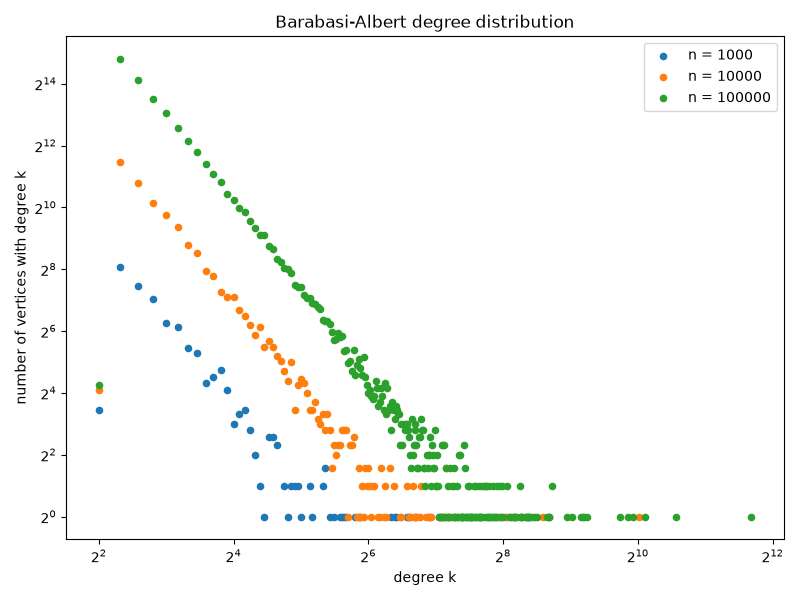
\includegraphics[width=0.8\textwidth]{plots/degree_dist.png}
    \caption{Degree distributions across different network sizes ($n = 1000, 10000, 100000$),
    plotted on log-log axes.}
    \label{fig:all_degree_distributions}
\end{figure}
The degree distribution was analyzed for $n = 1000$, $n = 10000$, and $n = 100000$
vertices, with each distribution overlaid on a single log-log plot. On these axes a
power law appears as a straight line, and all three sizes exhibit the same clear
linear trend, confirming \emph{scale free} behavior. The \textbf{heavy right skew}
characteristic of a power law is evident: a large number of low-degree vertices coexist
with a handful of very high-degree hubs (the tail extends past $k = 2^{10}$ for
$n = 100000$). As $n$ grows the distribution simply extends further along the same
slope, so the shape is preserved across scales. As such, the \emph{Barabasi-Albert}
random graphs follow a \textbf{power law}.






\subsection{Clustering Coefficients}


\subsubsection{Definition}

The clustering coefficient is
\[
    C = \frac{3 \cdot (\text{number of triangles})}{\text{number of 2-edge paths}}.
\]
The denominator is cheap; the numerator is computed via a degeneracy ordering so that
triangle counting runs in $O(d^2 n) = O(dm)$ expected time rather than the naïve $O(n^3)$.
\subsubsection{Psuedocode}
\begin{algorithm}
    \caption{Number of 2-Edge Paths}\label{alg:paths}
    \begin{algorithmic}[1]
        \Procedure{Num2EdgePaths}{$G$}
        \State $\text{total} \gets 0$
        \ForAll{$v \in G.V$}
            \State $d \gets \deg(v)$
            \State $\text{total} \gets \text{total} + \dfrac{d(d-1)}{2}$ \Comment{paths with $v$ in the middle}
        \EndFor
        \State \Return $\text{total}$
        \EndProcedure
    \end{algorithmic}
\end{algorithm}

\begin{algorithm}
    \caption{Degeneracy Ordering}\label{alg:degen}
    \begin{algorithmic}[1]
        \Procedure{DegeneracyOrdering}{$G$}
        \State $L \gets [\,]$, \quad $H_L \gets \varnothing$ \Comment{output ordering / vertices placed in $L$}
        \ForAll{$v \in G.V$}
            \State $d_v \gets \deg(v)$, \quad $N_v \gets [\,]$ \Comment{$N_v$: neighbors of $v$ before $v$ in $L$}
        \EndFor
        \ForAll{$v \in G.V$}
            \State $D[d_v] \gets D[d_v] \cup \{v\}$ \Comment{bucket vertices by current degree}
        \EndFor
        \State $k \gets 0$
        \For{$j \gets 1 \text{ to } n$}
            \State $i \gets \min\{\, i : D[i] \neq \varnothing \,\}$
            \State $k \gets \max(k, i)$
            \State $v \gets$ any vertex in $D[i]$
            \State $D[i] \gets D[i] \setminus \{v\}$
            \State prepend $v$ to $L$; \quad $H_L \gets H_L \cup \{v\}$
            \ForAll{$w \in G.\textsc{Neighbors}(v) \text{ with } w \notin H_L$}
                \State $D[d_w] \gets D[d_w] \setminus \{w\}$
                \State $d_w \gets d_w - 1$
                \State $D[d_w] \gets D[d_w] \cup \{w\}$
                \State append $w$ to $N_v$
            \EndFor
        \EndFor
        \State \Return $(L, N)$
        \EndProcedure
    \end{algorithmic}
\end{algorithm}

\begin{algorithm}
    \caption{Counting Triangles}\label{alg:tri}
    \begin{algorithmic}[1]
        \Procedure{CountTriangles}{$G$}
        \State $(L, N) \gets \textsc{DegeneracyOrdering}(G)$
        \State $\Delta \gets 0$
        \ForAll{$v \in L$}
            \ForAll{unordered pairs $\{u, w\} \subseteq N_v$}
                \If{$(u, w) \in E$} \Comment{$O(1)$ adjacency lookup}
                    \State $\Delta \gets \Delta + 1$
                \EndIf
            \EndFor
        \EndFor
        \State \Return $\Delta$
        \EndProcedure
    \end{algorithmic}
\end{algorithm}

\begin{algorithm}
    \caption{Clustering Coefficient}\label{alg:cc}
    \begin{algorithmic}[1]
        \Procedure{ClusteringCoefficient}{$G$}
        \State $\Delta \gets \textsc{CountTriangles}(G)$
        \State $P \gets \textsc{Num2EdgePaths}(G)$
        \State \Return $\dfrac{3\Delta}{P}$
        \EndProcedure
    \end{algorithmic}
\end{algorithm}







\subsubsection{Analysis}

\begin{figure}[H]
    \centering
    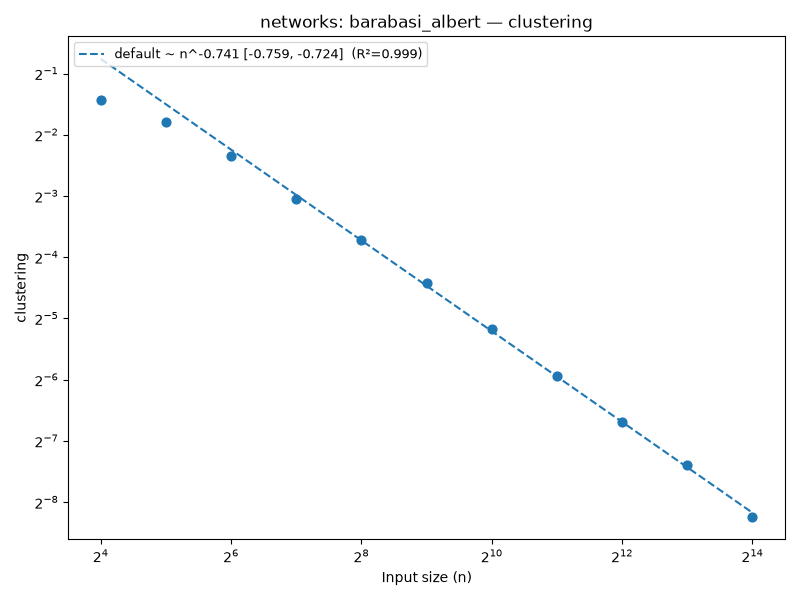
\includegraphics[width=0.9\textwidth]{plots/clustering.png}
    \caption{Average clustering vs $n$ (log-log axes) with a fitted power law.}
    \label{fig:cluster}
\end{figure}

The clustering coefficient, $\mcC$, measures how "cliquey" the network is. As shown
in Figure~\ref{fig:cluster}, as $n$ increases, $\mcC$ decreases. This makes sense,
since as we add more vertices via BA [\ref{alg:pa}], they \emph{still} form
connections to \emph{only} $d$ other vertices, but the denominator scales with $n$.

On log-log axes the measurements fall on a near-perfect straight line, so $\mcC$
follows a \textbf{power law} rather than an exponential. The fitted exponent is
\begin{equation*}
\mcC \propto n^{-0.74} \qquad (R^2 = 0.999)
\end{equation*}
The extremely tight fit ($R^2 = 0.999$) confirms that the decay is polynomial in $n$:
each doubling of the graph size multiplies the clustering coefficient by a constant
factor of $2^{-0.74} \approx 0.6$, so triangles become steadily rarer as the graph
grows but never vanish abruptly.

\subsection{Diameters}
\subsubsection{Definition}
The diameter, $d$, is the greatest distance between any pair of vertices, namely
\begin{equation*}
    d = \max_{v \in G.V}\max_{u \in G.V} d(v, u)
\end{equation*}
where $d \colon G.V \times G.V \rightarrow \bbR^+ \cup \{0\}$. 

\subsubsection{Psuedocode}

\begin{algorithm}
    \caption{Diameter}\label{alg:dh2}

    \begin{algorithmic}[1]
	    \Procedure{Hueristic II}{$G$}
        \State $r \gets \mathcal{U}(1, n)$ \Comment{A random vertex}
        \State $D_{\max} \gets 0$

        \While{ True }
            \State $(w, \text{dist}) \gets \text{BFS}(Graph, r)$
            \If{$\text{dist} > D_{\max}$}
                \State $D_{\max} \gets \text{dist}$
                \State $r \gets w$
            \Else
                \State \textbf{break}
            \EndIf
        \EndWhile
        
        \State \Return $D_{\max}$
	\EndProcedure
    \end{algorithmic}
    
\end{algorithm}

\subsubsection{Analysis}

\begin{figure}[H]
   \centering
   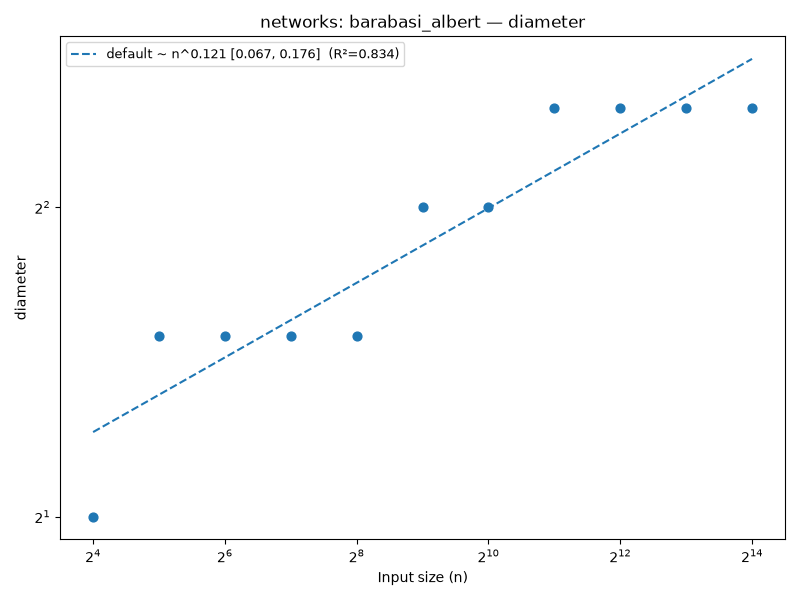
\includegraphics[width=0.8\textwidth]{plots/diameter.png}
   \caption{Average Diameter vs $n$ (log-log axes) with a fitted power law.}
   \label{fig:diam}
\end{figure}

As shown in Figure~\ref{fig:diam}, the average diameter increases with $n$, but only
very slowly: over roughly three orders of magnitude in $n$ the diameter barely triples.
Fitting a power law on log-log axes yields a tiny exponent,
\begin{equation*}
    d \propto n^{0.12} \qquad (R^2 = 0.834),
\end{equation*}
and such a small exponent with only a moderate fit is exactly the signature of
sub-polynomial, essentially \emph{logarithmic}, growth: preferential attachment
produces high-degree hubs that act as shortcuts, keeping pairwise distances short
even as the graph grows. The jagged, stair-step effect visible at certain values of
$n$ is an artifact of the diameter being integer-valued, since the average must
accumulate enough samples before incrementing to the next integer. As such, the
diameter \textbf{is changing as a function of $n$}, just far more slowly than any
power of $n$.


